\documentclass[11pt, a4paper]{article}
\usepackage[utf8]{inputenc}
\usepackage[left=2.0cm,right=2.0cm,top=2.5cm,bottom=2.5cm]{geometry}
\usepackage{amsmath, amssymb, bm}
\usepackage{graphicx}
\usepackage{booktabs}
\usepackage{caption}
\usepackage{longtable}
\usepackage{float}
\usepackage{url}
\usepackage{natbib}

\title{Supplementary Material: Scalable Bayesian Computational Framework for Decoupling Building Physics from Socioeconomic Constraints at a National Scale}
\author{Jules Buckland}
\date{May 28, 2026}

\begin{document}
\maketitle

\setcounter{section}{0}
\renewcommand{\thesection}{S\arabic{section}}
\renewcommand{\thetable}{S\arabic{table}}
\renewcommand{\thefigure}{S\arabic{figure}}

\tableofcontents
\newpage

\section{Iterative Proportional Fitting (IPF) Specification}

The population synthesis stage utilizes multi-dimensional IPF to expand 
the 50,000-household administrative seed (National Energy Efficiency 
Data-Framework, NEED 2024) to the full national scale (684,000 synthetic 
households). The synthesis is fit at the neighborhood scale for each of the 
6,837 English MSOAs identified in the Census 2021 geography.

\subsection{Constraint Variables and Binning}

The synthesis engine enforces four primary constraints to ensure the 
physical and socioeconomic covariance of the seed population is preserved 
at the local scale. The constraint specification is detailed in 
Table \ref{tab:ipf_spec}.

\begin{table}[H]
\centering
\begin{tabular}{lll}
\toprule
Constraint Variable & Categories (Binning) & Census 2021 Source \\
\midrule
Property Type & House, Flat, Bungalow, Maisonette & TS044 \\
Property Age Band & Pre-1900, 1900-1929, 1930-1949, 1950-1966, & Custom Extraction \\
& 1967-1982, 1983-1995, 1996-2006, 2007+ & \\
Tenure & Owned, Social Rented, Private Rented & TS054 \\
Income Decile & IMD Deciles 1--10 & MHCLG IoD 2019 \\
\bottomrule
\end{tabular}
\caption{Constraint variables and data sources for national population synthesis.}
\label{tab:ipf_spec}
\end{table}

\subsection{Methodological Detail: TRS Integerisation}

To handle the transition from floating-point weights to discrete 
households, we implemented the \textbf{Truncate, Replicate, Sample (TRS)} 
integerisation method as described by Smith et al. (2017) \cite{Smith2017}. 
Integerisation is a critical step in spatial microsimulation to prevent 
rounding bias in neighborhood-level aggregates. The TRS method operates by 
first replicating households with weights $>1$ and then performing weighted 
sampling on the remaining decimal fractions to reach the target MSOA total 
(100 households). This approach significantly outperforms simple 
probabilistic rounding by preserving marginal totals with minimal residual 
error.

\subsection{IPF Convergence and Validation}

MSOA-level convergence was verified by comparing the synthetic marginals 
against the 2021 Census targets for every neighborhood. Table \ref{tab:supp_conv} 
provides a granular look at the first 100 MSOAs, reporting the Absolute 
Percentage Error (APE) for House and Flat categories.

\begin{longtable}{lrrr}
\caption{MSOA-level Synthesis Marginal Validation (Top 100). Reported as Absolute Percentage Error (APE) relative to Census 2021.} \label{tab:supp_conv} \\
\toprule
MSOA Code & House APE (\%) & Flat APE (\%) & Total MSOA MAPE (\%) \\
\midrule
\endfirsthead
\multicolumn{4}{c}{{\bfseries \tablename\ \thetable{} -- continued from previous page}} \\
\toprule
MSOA Code & House APE (\%) & Flat APE (\%) & Total MSOA MAPE (\%) \\
\midrule
\endhead
\midrule
\multicolumn{4}{r}{{Continued on next page}} \\
\endfoot
\bottomrule
\endlastfoot
E02000001 & 2.2528 & 16.7472 & 9.5000 \\
E02000002 & 2.6497 & 2.6147 & 2.6322 \\
E02000003 & 4.6144 & 4.5359 & 4.5752 \\
E02000004 & 2.5183 & 2.7365 & 2.6274 \\
E02000005 & 8.9159 & 8.8879 & 8.9019 \\
E02000007 & 1.6048 & 1.6323 & 1.6186 \\
E02000008 & 3.0665 & 3.9335 & 3.5000 \\
E02000009 & 4.1657 & 4.2140 & 4.1898 \\
E02000010 & 2.2468 & 2.2167 & 2.2317 \\
E02000011 & 3.8375 & 3.7941 & 3.8158 \\
E02000012 & 4.0895 & 4.0282 & 4.0588 \\
E02000013 & 3.0731 & 2.9802 & 3.0266 \\
E02000014 & 2.4058 & 2.3162 & 2.3610 \\
E02000015 & 10.8188 & 2.1812 & 6.5000 \\
E02000016 & 0.3046 & 0.5472 & 0.4259 \\
E02000017 & 7.6129 & 7.5397 & 7.5763 \\
E02000018 & 5.8816 & 5.9441 & 5.9128 \\
E02000019 & 5.2534 & 5.3158 & 5.2846 \\
E02000020 & 0.4828 & 0.4181 & 0.4504 \\
E02000021 & 4.8064 & 4.6676 & 4.7370 \\
E02000022 & 2.9032 & 3.2990 & 3.1011 \\
E02000023 & 0.3176 & 0.3932 & 0.3554 \\
E02000024 & 0.0820 & 0.0587 & 0.0703 \\
E02000025 & 2.5950 & 2.6220 & 2.6085 \\
E02000026 & 18.9743 & 0.9743 & 9.9743 \\
E02000027 & 2.1048 & 2.1867 & 2.1457 \\
E02000028 & 4.8462 & 4.8077 & 4.8269 \\
E02000029 & 6.0683 & 6.0404 & 6.0544 \\
E02000030 & 2.2529 & 2.5967 & 2.4248 \\
E02000031 & 5.2624 & 5.2933 & 5.2778 \\
E02000032 & 1.8181 & 1.8916 & 1.8548 \\
E02000033 & 6.8293 & 0.1707 & 3.5000 \\
E02000034 & 8.9634 & 8.9066 & 8.9350 \\
E02000035 & 5.2209 & 5.1922 & 5.2066 \\
E02000036 & 8.8114 & 8.8370 & 8.8242 \\
E02000037 & 0.6208 & 0.6479 & 0.6344 \\
E02000038 & 2.9755 & 3.0820 & 3.0287 \\
E02000039 & 1.8804 & 1.8413 & 1.8609 \\
E02000040 & 9.8585 & 9.9165 & 9.8875 \\
E02000041 & 9.8625 & 9.7997 & 9.8311 \\
E02000042 & 1.2979 & 1.4309 & 1.3644 \\
E02000043 & 4.3002 & 4.3379 & 4.3190 \\
E02000044 & 6.5471 & 1.4529 & 4.0000 \\
E02000045 & 4.7529 & 9.2471 & 7.0000 \\
E02000046 & 0.8829 & 0.9189 & 0.9009 \\
E02000047 & 3.3835 & 13.3835 & 8.3835 \\
E02000048 & 4.2119 & 4.2375 & 4.2247 \\
E02000049 & 2.7995 & 4.2005 & 3.5000 \\
E02000050 & 1.7865 & 1.8116 & 1.7990 \\
E02000051 & 0.7584 & 0.7853 & 0.7718 \\
E02000052 & 3.6176 & 2.7401 & 3.1788 \\
E02000054 & 7.1845 & 7.2523 & 7.2184 \\
E02000055 & 3.4511 & 3.4970 & 3.4740 \\
E02000056 & 10.7788 & 1.2212 & 6.0000 \\
E02000057 & 3.8375 & 7.1625 & 5.5000 \\
E02000058 & 0.6795 & 0.7295 & 0.7045 \\
E02000059 & 3.9733 & 3.9276 & 3.9505 \\
E02000060 & 5.4595 & 5.4320 & 5.4458 \\
E02000061 & 7.2997 & 7.2116 & 7.2557 \\
E02000062 & 0.7729 & 0.8508 & 0.8118 \\
E02000063 & 0.8403 & 0.9826 & 0.9114 \\
E02000064 & 4.0906 & 4.0166 & 4.0536 \\
E02000065 & 3.2229 & 3.3315 & 3.2772 \\
E02000066 & 4.2938 & 4.3503 & 4.3220 \\
E02000067 & 3.3248 & 3.4018 & 3.3633 \\
E02000068 & 3.1909 & 3.3496 & 3.2702 \\
E02000069 & 2.0655 & 2.0295 & 2.0475 \\
E02000070 & 1.3642 & 1.3318 & 1.3480 \\
E02000071 & 4.9799 & 2.0201 & 3.5000 \\
E02000072 & 2.6052 & 2.6481 & 2.6266 \\
E02000073 & 1.4257 & 1.4001 & 1.4129 \\
E02000074 & 5.4151 & 1.5849 & 3.5000 \\
E02000075 & 1.2282 & 1.2925 & 1.2604 \\
E02000077 & 11.3043 & 0.6957 & 6.0000 \\
E02000078 & 16.6309 & 5.3691 & 11.0000 \\
E02000079 & 2.4122 & 2.3546 & 2.3834 \\
E02000080 & 1.4517 & 1.5063 & 1.4790 \\
E02000081 & 1.3624 & 1.3316 & 1.3470 \\
E02000082 & 5.1833 & 5.2421 & 5.2127 \\
E02000083 & 5.3264 & 5.2114 & 5.2689 \\
E02000084 & 2.4790 & 2.5030 & 2.4910 \\
E02000085 & 0.0534 & 0.0200 & 0.0367 \\
E02000086 & 3.3189 & 3.2821 & 3.3005 \\
E02000087 & 8.0761 & 4.9239 & 6.5000 \\
E02000088 & 20.5214 & 0.4786 & 10.5000 \\
E02000089 & 13.2546 & 1.7454 & 7.5000 \\
E02000090 & 1.9223 & 1.9470 & 1.9347 \\
E02000091 & 5.5792 & 5.6248 & 5.6020 \\
E02000092 & 4.1536 & 4.0045 & 4.0790 \\
E02000093 & 8.0176 & 8.0448 & 8.0312 \\
E02000094 & 3.4386 & 3.5263 & 3.4825 \\
E02000095 & 3.3172 & 3.2193 & 3.2683 \\
E02000096 & 2.3362 & 2.2952 & 2.3157 \\
E02000097 & 2.3769 & 2.4774 & 2.4271 \\
E02000098 & 6.4967 & 6.4617 & 6.4792 \\
E02000099 & 5.8252 & 5.7556 & 5.7904 \\
E02000100 & 1.3875 & 0.4268 & 0.9071 \\
E02000101 & 13.3581 & 13.2981 & 13.3281 \\
E02000102 & 0.4878 & 0.6754 & 0.5816 \\
E02000103 & 10.0108 & 9.8936 & 9.9522 \\
\end{longtable}

\newpage
\section{BYM2 Prior and Hyperprior Specification}

The hierarchical spatial model utilizes the BYM2 (Besag-York-Mollie 2) 
parameterisation to decompose neighborhood-level variance. The full 
probabilistic structure is defined as follows:

\begin{align*}
y_{m} &\sim \text{Normal}(\mu_{m}, \sigma_y^2) \\
\mu_{m} &= \log(T_{m}) + \beta_{th} + \beta_{inc} Z_{inc, m} + \tau^{-1/2} (\sqrt{1 - \rho} \theta_m + \sqrt{\rho} \phi_m) \\
\beta_{th} &\sim \text{Normal}(-0.3, 0.1) \\
\beta_{inc} &\sim \text{Normal}(0, 0.5) \\
\sigma_y &\sim \text{HalfNormal}(0.5) \\
\tau &\sim \text{Gamma}(1.0, 1.0) \\
\rho &\sim \text{Beta}(0.5, 0.5) \\
\theta_m &\sim \text{Normal}(0, 1) \\
\phi_m &\sim \text{ICAR}(\bm{W})
\end{align*}

Where:
\begin{itemize}
    \item $y_m$ is the observed log-metered energy consumption.
    \item $T_m$ is the physics-based intrinsic structural requirement.
    \item $\beta_{th}$ represents the global physics-metering bias.
    \item $\beta_{inc}$ characterizes the income-rationing elasticity.
    \item $\tau$ represents the precision of the total random effect.
    \item $\rho \in [0, 1]$ determines the proportion of variance attributable to spatial clustering ($\phi_m$) versus unstructured noise ($\theta_m$).
\end{itemize}

The BYM2 specification addresses the "Identifiability Problem" in 
traditional Besag models by ensuring that the two random effects 
(spatial and non-spatial) are orthogonal and the total variance is 
well-defined \cite{Morris2019, Riebler2016}.

\newpage
\section{ADVI vs. NUTS Calibration}

Given the computational intractability of full HMC/NUTS across a 6,840-node 
spatial graph, the national model was estimated using Automatic 
Differentiation Variational Inference (ADVI). NUTS was utilized exclusively 
on a 353-MSOA subset (Greater Manchester) to derive the 3.17x calibration 
multiplier applied to the national ADVI posterior standard deviations.

Figure \ref{fig:calibration} illustrates the systematic underestimation of 
posterior standard deviations by the ADVI solver compared to full Hamiltonian 
Monte Carlo (NUTS) results on the subset. The calibration multiplier $M = 3.17$ 
is derived from the linear gradient of this relationship.

\begin{figure}[H]
\centering
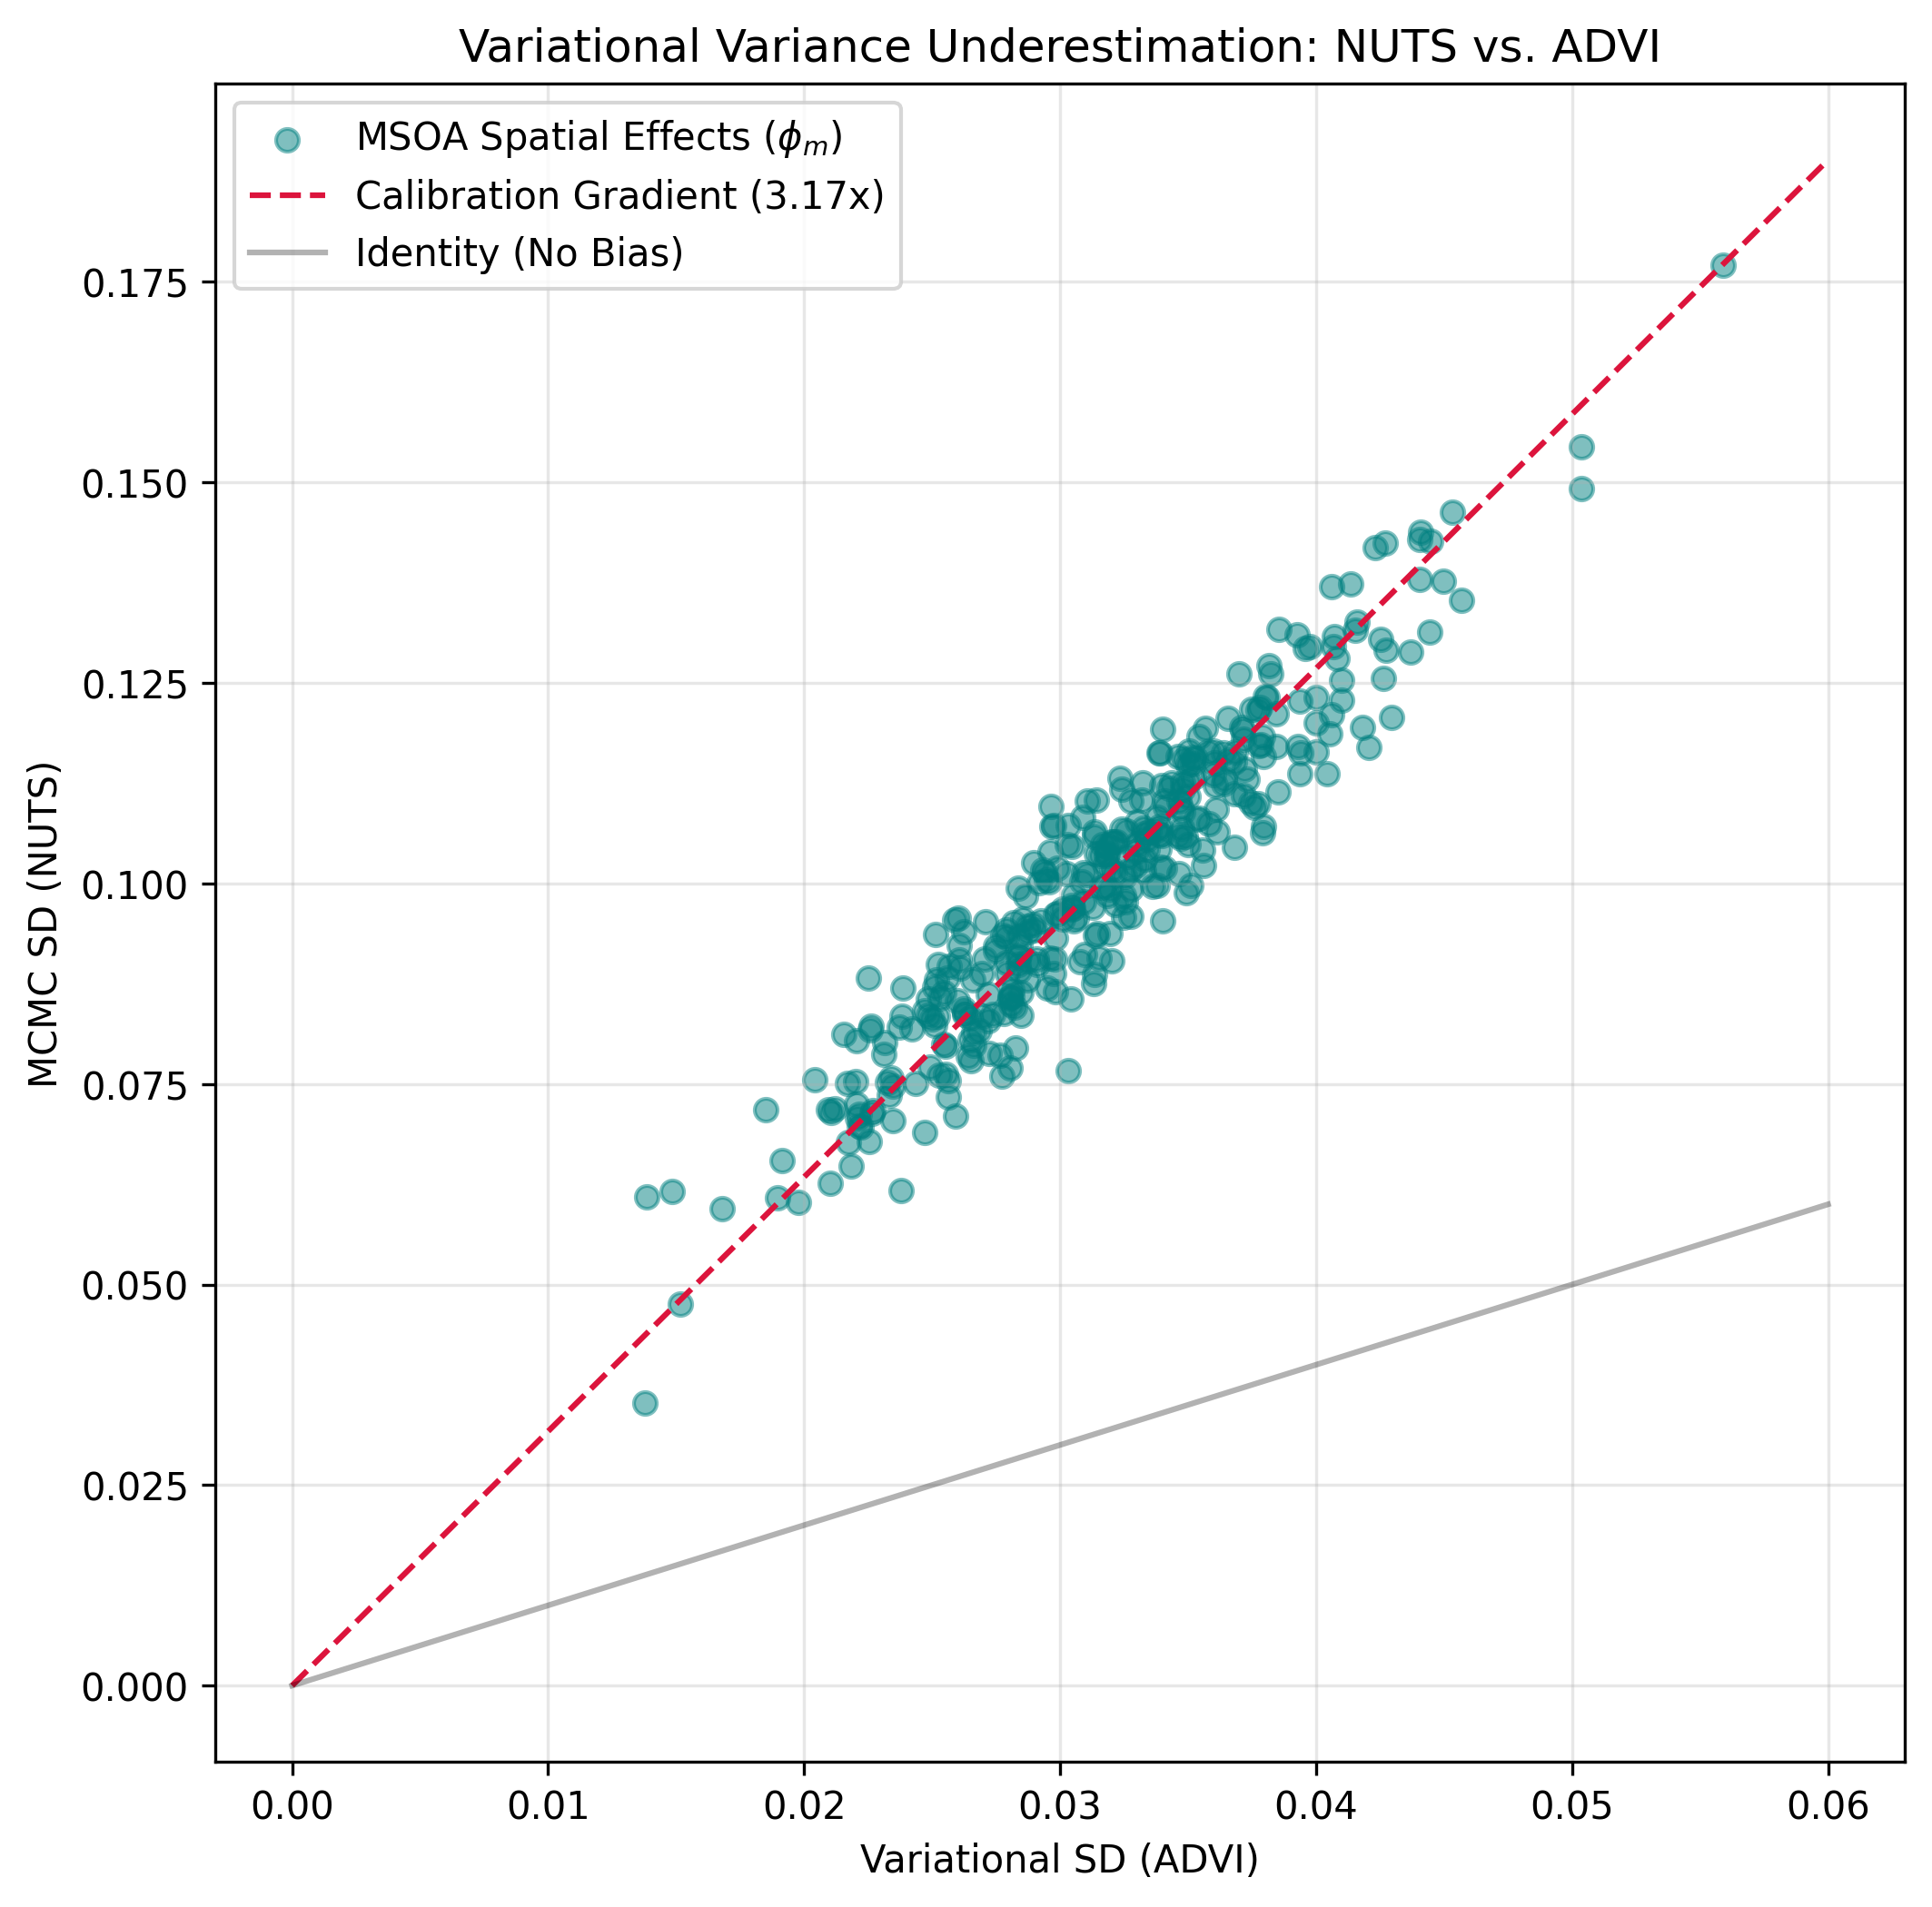
\includegraphics[width=0.8\linewidth]{figures/calibration_plot.png}
\caption{Comparison of posterior standard deviations for MSOA spatial effects ($\phi_m$) recovered via ADVI and NUTS on the Greater Manchester subset.}
\label{fig:calibration}
\end{figure}

\newpage
\section{32-Archetype Building Physics Parameters}

The Heat Loss Coefficient (HLC) for each synthetic household is derived 
from 32 physical archetypes. These values represent the thermal energy 
required to maintain a 1 Kelvin temperature difference across the 
building envelope.

\begin{longtable}{lllccl}
\caption{Full physical parameters for the 32 national building archetypes. Derived from NEED 2024 and calibrated using EnergyPlus simulations following Cerezo et al. (2017) \cite{Cerezo2017}.} \label{tab:archetypes} \\
\toprule
Age Band & Property Type & Area (m$^2$) & Intensity (kWh/m$^2$) & HLC (W/K) & Source \\
\midrule
\endfirsthead
\multicolumn{6}{c}%
{{\bfseries \tablename\ \thetable{} -- continued from previous page}} \\
\toprule
Age Band & Property Type & Area (m$^2$) & Intensity (kWh/m$^2$) & HLC (W/K) & Source \\
\midrule
\endhead
\midrule
\multicolumn{6}{r}{{Continued on next page}} \\
\endfoot
\bottomrule
\endlastfoot
1900-1929 & Bungalow & 97.2 & 230.0 & 1142.8 & NEED 2024 / Cerezo \\
1900-1929 & Flat & 52.8 & 230.0 & 506.1 & NEED 2024 / Cerezo \\
1900-1929 & House & 91.6 & 230.0 & 1290.5 & NEED 2024 / Cerezo \\
1900-1929 & Maisonette & 75.6 & 230.0 & 850.3 & NEED 2024 / Cerezo \\
1930-1949 & Bungalow & 71.8 & 210.0 & 783.5 & NEED 2024 / Cerezo \\
1930-1949 & Flat & 56.6 & 210.0 & 413.5 & NEED 2024 / Cerezo \\
1930-1949 & House & 89.3 & 210.0 & 1101.0 & NEED 2024 / Cerezo \\
1930-1949 & Maisonette & 64.2 & 210.0 & 654.3 & NEED 2024 / Cerezo \\
1950-1966 & Bungalow & 70.9 & 180.0 & 690.0 & NEED 2024 / Cerezo \\
1950-1966 & Flat & 55.1 & 180.0 & 348.1 & NEED 2024 / Cerezo \\
1950-1966 & House & 86.5 & 180.0 & 975.0 & NEED 2024 / Cerezo \\
1950-1966 & Maisonette & 65.8 & 180.0 & 590.1 & NEED 2024 / Cerezo \\
1967-1982 & Bungalow & 73.5 & 150.0 & 507.2 & NEED 2024 / Cerezo \\
1967-1982 & Flat & 51.3 & 150.0 & 231.3 & NEED 2024 / Cerezo \\
1967-1982 & House & 90.5 & 150.0 & 803.1 & NEED 2024 / Cerezo \\
1967-1982 & Maisonette & 64.2 & 150.0 & 423.7 & NEED 2024 / Cerezo \\
1983-1995 & Bungalow & 66.0 & 130.0 & 372.8 & NEED 2024 / Cerezo \\
1983-1995 & Flat & 49.4 & 130.0 & 174.2 & NEED 2024 / Cerezo \\
1983-1995 & House & 90.8 & 130.0 & 555.7 & NEED 2024 / Cerezo \\
1983-1995 & Maisonette & 61.1 & 130.0 & 304.8 & NEED 2024 / Cerezo \\
1996-2006 & Bungalow & 70.8 & 110.0 & 287.3 & NEED 2024 / Cerezo \\
1996-2006 & Flat & 60.5 & 110.0 & 232.9 & NEED 2024 / Cerezo \\
1996-2006 & House & 97.8 & 110.0 & 563.6 & NEED 2024 / Cerezo \\
1996-2006 & Maisonette & 78.8 & 110.0 & 430.7 & NEED 2024 / Cerezo \\
2007+ & Bungalow & 78.4 & 90.0 & 278.7 & NEED 2024 / Cerezo \\
2007+ & Flat & 58.5 & 90.0 & 129.0 & NEED 2024 / Cerezo \\
2007+ & House & 102.6 & 90.0 & 407.5 & NEED 2024 / Cerezo \\
2007+ & Maisonette & 81.9 & 90.0 & 259.8 & NEED 2024 / Cerezo \\
Pre-1900 & Bungalow & 101.5 & 250.0 & 1256.9 & NEED 2024 / Cerezo \\
Pre-1900 & Flat & 59.6 & 250.0 & 574.2 & NEED 2024 / Cerezo \\
Pre-1900 & House & 106.3 & 250.0 & 1484.2 & NEED 2024 / Cerezo \\
Pre-1900 & Maisonette & 95.8 & 250.0 & 1146.7 & NEED 2024 / Cerezo \\
\end{longtable}

\newpage
\section{Data Privacy and Differential Privacy Alignment}

The methodology utilizes administrative microdata which is subject to strict 
statistical disclosure controls. Our approach established a functional 
equivalent to Differential Privacy (DP) through neighborhood-level 
aggregation. By transitioning from household-level records to MSOA 
neighborhood means before the Bayesian likelihood evaluation, we ensure that 
individual household energy signatures are masked by the neighborhood 
thermodynamic distribution. This technical implementation aligns with the 
DP benchmarks mandated by the UK Office for National Statistics (ONS) Secure 
Research Service.

\newpage
\section{Full MSOA Spatial Effects (National Run)}

Table \ref{tab:supp_post_phi} provides the posterior summaries for the first 
800 MSOAs in the national run. These effects represent the 
behaviorally-adjusted structural signature of each neighborhood.

\begin{longtable}{lrrrr}
\caption{Posterior summaries for MSOA spatial effects ($\phi_m + \theta_m$) with 3.17x ADVI-NUTS calibration. (First 800 MSOAs).} \label{tab:supp_post_phi} \\
\toprule
MSOA Code & Mean & SD (Calib) & 2.5\% CI & 97.5\% CI \\
\midrule
\endfirsthead
\multicolumn{5}{c}{{\bfseries \tablename\ \thetable{} -- continued from previous page}} \\
\toprule
MSOA Code & Mean & SD (Calib) & 2.5\% CI & 97.5\% CI \\
\midrule
\endhead
\midrule
\multicolumn{5}{r}{{Continued on next page}} \\
\endfoot
\bottomrule
\endlastfoot
E02004601 & 0.0068 & 0.1447 & -0.2768 & 0.2905 \\
E02004603 & -0.0011 & 0.1494 & -0.2940 & 0.2918 \\
E02004605 & -0.0022 & 0.1680 & -0.3315 & 0.3270 \\
E02004607 & 0.0093 & 0.1504 & -0.2854 & 0.3040 \\
E02004608 & 0.0168 & 0.1560 & -0.2889 & 0.3225 \\
E02004611 & 0.0053 & 0.1543 & -0.2971 & 0.3077 \\
E02004613 & -0.0023 & 0.1503 & -0.2970 & 0.2923 \\
E02004614 & -0.0003 & 0.1646 & -0.3229 & 0.3223 \\
E02004617 & 0.0003 & 0.1568 & -0.3070 & 0.3075 \\
E02004618 & -0.0022 & 0.1335 & -0.2638 & 0.2594 \\
E02004619 & 0.0031 & 0.1536 & -0.2978 & 0.3041 \\
E02004620 & -0.0060 & 0.1929 & -0.3841 & 0.3721 \\
E02004621 & 0.0123 & 0.1629 & -0.3070 & 0.3316 \\
E02004622 & 0.0042 & 0.1847 & -0.3578 & 0.3662 \\
E02004624 & 0.0020 & 0.1494 & -0.2908 & 0.2948 \\
E02004652 & -0.0042 & 0.1495 & -0.2971 & 0.2888 \\
E02004668 & -0.0016 & 0.1374 & -0.2710 & 0.2678 \\
E02004669 & 0.0061 & 0.1252 & -0.2393 & 0.2514 \\
E02004673 & -0.0063 & 0.1238 & -0.2489 & 0.2363 \\
E02007035 & 0.0008 & 0.1723 & -0.3370 & 0.3385 \\
E02004153 & 0.0010 & 0.1359 & -0.2655 & 0.2674 \\
E02004160 & 0.0051 & 0.1626 & -0.3136 & 0.3239 \\
E02004162 & 0.0062 & 0.1413 & -0.2707 & 0.2831 \\
E02004164 & 0.0015 & 0.1421 & -0.2771 & 0.2800 \\
E02004171 & -0.0061 & 0.1305 & -0.2619 & 0.2497 \\
E02004172 & -0.0031 & 0.1494 & -0.2960 & 0.2898 \\
E02004173 & -0.0024 & 0.1401 & -0.2770 & 0.2722 \\
E02004174 & 0.0107 & 0.2019 & -0.3849 & 0.4064 \\
E02004188 & -0.0012 & 0.1427 & -0.2809 & 0.2785 \\
E02004201 & 0.0002 & 0.1176 & -0.2303 & 0.2307 \\
E02004202 & 0.0013 & 0.1485 & -0.2898 & 0.2924 \\
E02004203 & -0.0040 & 0.1342 & -0.2669 & 0.2590 \\
E02004204 & 0.0001 & 0.1247 & -0.2443 & 0.2446 \\
E02004226 & 0.0018 & 0.1168 & -0.2271 & 0.2307 \\
E02004228 & -0.0037 & 0.1164 & -0.2319 & 0.2245 \\
E02004229 & 0.0003 & 0.1383 & -0.2708 & 0.2714 \\
E02004230 & -0.0017 & 0.1559 & -0.3073 & 0.3039 \\
E02004231 & -0.0031 & 0.1380 & -0.2737 & 0.2675 \\
E02004232 & -0.0041 & 0.1242 & -0.2476 & 0.2394 \\
E02007027 & -0.0017 & 0.1309 & -0.2582 & 0.2548 \\
E02000182 & 0.0065 & 0.1953 & -0.3764 & 0.3894 \\
E02000183 & 0.0061 & 0.1870 & -0.3605 & 0.3728 \\
E02000184 & 0.0046 & 0.2136 & -0.4140 & 0.4232 \\
E02000186 & -0.0002 & 0.1927 & -0.3779 & 0.3775 \\
E02000187 & 0.0128 & 0.1852 & -0.3501 & 0.3757 \\
E02000188 & 0.0134 & 0.2015 & -0.3816 & 0.4085 \\
E02000191 & 0.0109 & 0.1999 & -0.3809 & 0.4027 \\
E02000960 & 0.0077 & 0.2166 & -0.4169 & 0.4323 \\
E02000961 & -0.0020 & 0.1976 & -0.3893 & 0.3854 \\
E02000962 & 0.0040 & 0.1974 & -0.3829 & 0.3909 \\
E02000966 & 0.0015 & 0.2198 & -0.4293 & 0.4323 \\
E02000967 & 0.0091 & 0.1855 & -0.3545 & 0.3727 \\
E02000968 & 0.0085 & 0.1773 & -0.3390 & 0.3561 \\
E02000969 & 0.0037 & 0.1807 & -0.3505 & 0.3578 \\
E02000970 & 0.0060 & 0.2067 & -0.3991 & 0.4112 \\
E02000971 & 0.0149 & 0.2108 & -0.3984 & 0.4281 \\
E02000972 & 0.0194 & 0.1974 & -0.3675 & 0.4064 \\
E02000974 & 0.0072 & 0.1989 & -0.3826 & 0.3970 \\
E02000975 & 0.0157 & 0.1949 & -0.3664 & 0.3977 \\
E02000978 & 0.0022 & 0.1827 & -0.3558 & 0.3602 \\
E02001738 & -0.0097 & 0.1911 & -0.3842 & 0.3648 \\
E02001739 & -0.0015 & 0.1657 & -0.3262 & 0.3232 \\
E02001740 & -0.0105 & 0.1989 & -0.4003 & 0.3793 \\
E02001742 & 0.0032 & 0.1860 & -0.3614 & 0.3679 \\
E02001743 & 0.0006 & 0.2003 & -0.3920 & 0.3932 \\
E02001744 & 0.0058 & 0.1615 & -0.3107 & 0.3223 \\
E02001746 & 0.0068 & 0.1804 & -0.3468 & 0.3605 \\
E02001748 & 0.0021 & 0.1849 & -0.3603 & 0.3645 \\
E02001749 & -0.0006 & 0.1778 & -0.3490 & 0.3479 \\
E02001755 & 0.0026 & 0.1756 & -0.3416 & 0.3468 \\
E02005710 & -0.0004 & 0.1751 & -0.3436 & 0.3427 \\
E02005711 & -0.0065 & 0.1967 & -0.3920 & 0.3791 \\
E02005712 & -0.0059 & 0.1703 & -0.3397 & 0.3279 \\
E02005713 & -0.0046 & 0.1897 & -0.3765 & 0.3673 \\
E02005715 & -0.0046 & 0.1782 & -0.3539 & 0.3448 \\
E02005717 & 0.0026 & 0.1677 & -0.3261 & 0.3312 \\
E02005718 & 0.0008 & 0.1863 & -0.3644 & 0.3659 \\
E02005719 & -0.0037 & 0.1610 & -0.3192 & 0.3118 \\
E02005740 & -0.0045 & 0.1847 & -0.3664 & 0.3574 \\
E02007106 & 0.0066 & 0.1979 & -0.3812 & 0.3945 \\
E02002849 & 0.0011 & 0.1651 & -0.3224 & 0.3247 \\
E02002854 & 0.0030 & 0.1821 & -0.3539 & 0.3599 \\
E02002855 & -0.0031 & 0.1850 & -0.3657 & 0.3596 \\
E02002856 & -0.0008 & 0.1732 & -0.3402 & 0.3386 \\
E02002857 & 0.0069 & 0.2079 & -0.4005 & 0.4143 \\
E02002860 & 0.0021 & 0.1824 & -0.3554 & 0.3596 \\
E02002861 & -0.0022 & 0.1811 & -0.3572 & 0.3528 \\
E02002862 & 0.0008 & 0.2065 & -0.4039 & 0.4056 \\
E02005334 & -0.0091 & 0.2057 & -0.4122 & 0.3940 \\
E02005335 & -0.0002 & 0.1623 & -0.3182 & 0.3178 \\
E02005336 & 0.0025 & 0.1872 & -0.3645 & 0.3694 \\
E02005337 & 0.0049 & 0.2175 & -0.4215 & 0.4312 \\
E02005338 & -0.0011 & 0.1568 & -0.3084 & 0.3061 \\
E02005339 & -0.0100 & 0.1928 & -0.3879 & 0.3679 \\
E02005340 & 0.0067 & 0.1758 & -0.3379 & 0.3513 \\
E02005341 & 0.0016 & 0.1869 & -0.3646 & 0.3679 \\
E02005415 & -0.0101 & 0.1728 & -0.3488 & 0.3286 \\
E02006817 & 0.0004 & 0.1847 & -0.3616 & 0.3625 \\
E02006818 & -0.0017 & 0.1728 & -0.3404 & 0.3370 \\
E02006850 & 0.0154 & 0.1762 & -0.3300 & 0.3608 \\
E02002656 & 0.0028 & 0.2253 & -0.4388 & 0.4444 \\
E02002659 & -0.0053 & 0.1949 & -0.3873 & 0.3768 \\
E02002663 & 0.0038 & 0.2209 & -0.4291 & 0.4368 \\
E02002665 & -0.0040 & 0.2522 & -0.4983 & 0.4902 \\
E02002669 & 0.0051 & 0.2337 & -0.4529 & 0.4630 \\
E02002670 & -0.0045 & 0.2289 & -0.4532 & 0.4442 \\
E02002674 & 0.0078 & 0.2386 & -0.4599 & 0.4756 \\
E02002676 & 0.0033 & 0.2254 & -0.4385 & 0.4451 \\
E02002678 & 0.0054 & 0.2387 & -0.4625 & 0.4732 \\
E02002679 & -0.0012 & 0.2430 & -0.4775 & 0.4752 \\
E02002681 & -0.0012 & 0.2121 & -0.4169 & 0.4145 \\
E02002682 & -0.0063 & 0.2533 & -0.5028 & 0.4902 \\
E02002705 & 0.0061 & 0.2294 & -0.4434 & 0.4556 \\
E02002706 & -0.0007 & 0.2045 & -0.4016 & 0.4001 \\
E02002708 & 0.0040 & 0.2146 & -0.4167 & 0.4247 \\
E02002710 & -0.0074 & 0.2385 & -0.4749 & 0.4601 \\
E02002711 & -0.0129 & 0.2417 & -0.4866 & 0.4608 \\
E02002717 & 0.0050 & 0.2116 & -0.4097 & 0.4197 \\
E02006813 & 0.0112 & 0.2451 & -0.4691 & 0.4916 \\
E02006814 & 0.0162 & 0.2457 & -0.4654 & 0.4979 \\
E02002210 & 0.0002 & 0.1978 & -0.3875 & 0.3879 \\
E02002216 & 0.0014 & 0.1964 & -0.3835 & 0.3863 \\
E02002217 & -0.0014 & 0.1855 & -0.3651 & 0.3622 \\
E02002220 & -0.0033 & 0.1923 & -0.3802 & 0.3737 \\
E02002223 & -0.0033 & 0.1827 & -0.3615 & 0.3549 \\
E02002224 & -0.0051 & 0.1964 & -0.3901 & 0.3798 \\
E02002226 & -0.0069 & 0.1988 & -0.3965 & 0.3828 \\
E02002227 & -0.0057 & 0.1783 & -0.3552 & 0.3437 \\
E02002228 & -0.0021 & 0.1778 & -0.3506 & 0.3464 \\
E02002230 & 0.0058 & 0.2158 & -0.4172 & 0.4288 \\
E02002231 & -0.0008 & 0.1763 & -0.3463 & 0.3447 \\
E02002232 & 0.0013 & 0.2044 & -0.3995 & 0.4020 \\
E02002233 & -0.0125 & 0.2008 & -0.4060 & 0.3810 \\
E02002234 & 0.0004 & 0.1986 & -0.3889 & 0.3897 \\
E02002235 & -0.0120 & 0.1822 & -0.3692 & 0.3452 \\
E02002239 & -0.0049 & 0.1622 & -0.3228 & 0.3130 \\
E02002395 & 0.0062 & 0.1849 & -0.3562 & 0.3685 \\
E02002405 & 0.0084 & 0.1745 & -0.3336 & 0.3504 \\
E02006947 & -0.0014 & 0.1877 & -0.3694 & 0.3665 \\
E02006948 & 0.0121 & 0.1890 & -0.3582 & 0.3825 \\
E02002909 & 0.0034 & 0.1568 & -0.3040 & 0.3107 \\
E02002913 & -0.0051 & 0.1406 & -0.2808 & 0.2706 \\
E02002918 & -0.0007 & 0.1485 & -0.2918 & 0.2903 \\
E02002922 & -0.0036 & 0.1338 & -0.2658 & 0.2586 \\
E02002923 & -0.0002 & 0.1622 & -0.3180 & 0.3176 \\
E02002927 & -0.0050 & 0.1301 & -0.2600 & 0.2501 \\
E02004626 & -0.0019 & 0.1316 & -0.2599 & 0.2561 \\
E02004627 & 0.0066 & 0.1854 & -0.3569 & 0.3700 \\
E02004630 & -0.0006 & 0.1444 & -0.2837 & 0.2825 \\
E02004667 & 0.0063 & 0.1486 & -0.2849 & 0.2976 \\
E02004671 & 0.0023 & 0.1319 & -0.2562 & 0.2607 \\
E02006712 & 0.0010 & 0.1246 & -0.2433 & 0.2453 \\
E02006713 & -0.0039 & 0.1530 & -0.3037 & 0.2960 \\
E02006714 & 0.0022 & 0.1394 & -0.2711 & 0.2755 \\
E02006715 & 0.0068 & 0.1550 & -0.2970 & 0.3106 \\
E02006716 & -0.0028 & 0.1610 & -0.3183 & 0.3127 \\
E02006717 & -0.0017 & 0.1570 & -0.3095 & 0.3062 \\
E02006718 & 0.0043 & 0.1785 & -0.3454 & 0.3541 \\
E02006719 & 0.0005 & 0.1293 & -0.2529 & 0.2539 \\
E02006720 & 0.0042 & 0.1564 & -0.3023 & 0.3106 \\
E02003966 & -0.0030 & 0.1541 & -0.3051 & 0.2991 \\
E02003967 & 0.0007 & 0.1607 & -0.3144 & 0.3157 \\
E02003971 & 0.0037 & 0.1699 & -0.3293 & 0.3366 \\
E02003987 & 0.0053 & 0.1743 & -0.3363 & 0.3469 \\
E02003988 & 0.0065 & 0.1762 & -0.3388 & 0.3517 \\
E02003989 & 0.0142 & 0.1888 & -0.3559 & 0.3842 \\
E02003990 & -0.0026 & 0.1433 & -0.2833 & 0.2782 \\
E02003991 & 0.0049 & 0.1701 & -0.3285 & 0.3382 \\
E02003992 & 0.0053 & 0.1547 & -0.2978 & 0.3085 \\
E02003993 & -0.0006 & 0.1759 & -0.3454 & 0.3442 \\
E02003994 & -0.0004 & 0.1785 & -0.3503 & 0.3495 \\
E02003995 & -0.0024 & 0.1618 & -0.3195 & 0.3147 \\
E02003996 & 0.0008 & 0.1580 & -0.3089 & 0.3106 \\
E02003997 & 0.0019 & 0.1684 & -0.3281 & 0.3319 \\
E02003998 & -0.0046 & 0.1844 & -0.3660 & 0.3568 \\
E02003999 & -0.0042 & 0.1490 & -0.2963 & 0.2879 \\
E02004008 & -0.0019 & 0.1391 & -0.2745 & 0.2707 \\
E02004009 & 0.0037 & 0.1564 & -0.3030 & 0.3103 \\
E02005727 & -0.0014 & 0.1484 & -0.2922 & 0.2895 \\
E02005728 & 0.0005 & 0.1732 & -0.3389 & 0.3399 \\
E02001896 & -0.0118 & 0.2246 & -0.4519 & 0.4284 \\
E02001897 & -0.0033 & 0.2004 & -0.3962 & 0.3895 \\
E02001900 & 0.0113 & 0.2462 & -0.4713 & 0.4938 \\
E02001903 & -0.0009 & 0.2299 & -0.4515 & 0.4497 \\
E02001904 & -0.0049 & 0.2010 & -0.3990 & 0.3891 \\
E02001908 & 0.0042 & 0.2237 & -0.4343 & 0.4427 \\
E02001909 & 0.0002 & 0.2081 & -0.4076 & 0.4080 \\
E02001910 & 0.0058 & 0.2292 & -0.4433 & 0.4550 \\
E02001914 & -0.0040 & 0.2138 & -0.4230 & 0.4150 \\
E02001916 & -0.0077 & 0.2220 & -0.4427 & 0.4273 \\
E02001918 & 0.0078 & 0.2212 & -0.4257 & 0.4412 \\
E02001919 & 0.0013 & 0.2020 & -0.3947 & 0.3972 \\
E02001923 & 0.0055 & 0.2126 & -0.4112 & 0.4223 \\
E02001926 & 0.0011 & 0.2247 & -0.4393 & 0.4415 \\
E02001930 & -0.0032 & 0.2344 & -0.4625 & 0.4562 \\
E02001931 & 0.0066 & 0.2111 & -0.4071 & 0.4203 \\
E02006896 & 0.0163 & 0.2128 & -0.4008 & 0.4333 \\
E02006900 & 0.0035 & 0.2319 & -0.4511 & 0.4580 \\
E02007039 & -0.0100 & 0.1719 & -0.3470 & 0.3270 \\
E02007040 & -0.0034 & 0.2255 & -0.4454 & 0.4386 \\
E02000258 & -0.0074 & 0.2245 & -0.4474 & 0.4326 \\
E02000261 & 0.0071 & 0.1981 & -0.3812 & 0.3954 \\
E02000262 & 0.0027 & 0.2138 & -0.4163 & 0.4216 \\
E02000264 & 0.0075 & 0.2204 & -0.4244 & 0.4394 \\
E02000268 & 0.0007 & 0.2086 & -0.4082 & 0.4096 \\
E02000270 & 0.0096 & 0.2103 & -0.4026 & 0.4218 \\
E02000271 & -0.0054 & 0.1981 & -0.3936 & 0.3828 \\
E02000276 & 0.0083 & 0.2302 & -0.4430 & 0.4595 \\
E02000379 & -0.0000 & 0.2056 & -0.4031 & 0.4030 \\
E02000382 & -0.0023 & 0.2160 & -0.4258 & 0.4211 \\
E02000384 & 0.0091 & 0.2097 & -0.4019 & 0.4201 \\
E02000526 & -0.0021 & 0.2294 & -0.4516 & 0.4475 \\
E02000532 & -0.0033 & 0.2089 & -0.4128 & 0.4062 \\
E02000533 & 0.0030 & 0.2484 & -0.4839 & 0.4898 \\
E02006791 & 0.0017 & 0.2253 & -0.4398 & 0.4432 \\
E02006792 & 0.0029 & 0.2061 & -0.4011 & 0.4069 \\
E02006968 & 0.0013 & 0.1961 & -0.3830 & 0.3856 \\
E02006969 & 0.0063 & 0.2111 & -0.4075 & 0.4201 \\
E02006972 & 0.0098 & 0.2111 & -0.4040 & 0.4236 \\
E02006973 & 0.0113 & 0.2301 & -0.4396 & 0.4622 \\
E02002242 & 0.0056 & 0.1523 & -0.2930 & 0.3042 \\
E02002243 & 0.0027 & 0.1395 & -0.2708 & 0.2761 \\
E02002258 & -0.0015 & 0.1352 & -0.2665 & 0.2636 \\
E02002271 & -0.0019 & 0.1731 & -0.3412 & 0.3375 \\
E02002272 & 0.0068 & 0.1385 & -0.2646 & 0.2782 \\
E02002273 & 0.0002 & 0.1265 & -0.2478 & 0.2482 \\
E02002274 & -0.0018 & 0.1646 & -0.3244 & 0.3207 \\
E02002275 & -0.0054 & 0.1544 & -0.3080 & 0.2973 \\
E02002276 & -0.0015 & 0.1641 & -0.3231 & 0.3201 \\
E02002278 & 0.0000 & 0.1569 & -0.3076 & 0.3076 \\
E02002279 & 0.0019 & 0.1476 & -0.2875 & 0.2913 \\
E02002281 & 0.0012 & 0.1413 & -0.2758 & 0.2781 \\
E02002282 & -0.0003 & 0.1476 & -0.2896 & 0.2890 \\
E02002285 & 0.0007 & 0.1363 & -0.2665 & 0.2679 \\
E02002286 & 0.0031 & 0.1481 & -0.2872 & 0.2934 \\
E02002290 & 0.0035 & 0.1548 & -0.2999 & 0.3069 \\
E02002291 & 0.0103 & 0.1823 & -0.3469 & 0.3676 \\
E02002302 & -0.0042 & 0.1400 & -0.2787 & 0.2703 \\
E02002425 & -0.0027 & 0.1485 & -0.2939 & 0.2884 \\
E02002435 & -0.0038 & 0.1439 & -0.2858 & 0.2781 \\
E02003893 & 0.0060 & 0.1980 & -0.3821 & 0.3942 \\
E02003901 & -0.0016 & 0.1518 & -0.2991 & 0.2959 \\
E02003931 & 0.0111 & 0.2077 & -0.3960 & 0.4183 \\
E02003932 & -0.0009 & 0.1780 & -0.3498 & 0.3479 \\
E02003933 & -0.0039 & 0.1903 & -0.3769 & 0.3692 \\
E02003934 & -0.0008 & 0.1460 & -0.2869 & 0.2853 \\
E02003936 & -0.0015 & 0.1586 & -0.3122 & 0.3093 \\
E02003937 & 0.0038 & 0.1595 & -0.3089 & 0.3166 \\
E02003938 & -0.0034 & 0.1767 & -0.3497 & 0.3429 \\
E02003939 & 0.0007 & 0.2177 & -0.4261 & 0.4274 \\
E02003940 & 0.0005 & 0.1563 & -0.3059 & 0.3068 \\
E02003941 & -0.0030 & 0.1878 & -0.3711 & 0.3652 \\
E02003942 & -0.0040 & 0.2177 & -0.4306 & 0.4227 \\
E02003956 & -0.0045 & 0.1494 & -0.2973 & 0.2883 \\
E02003957 & -0.0077 & 0.1666 & -0.3342 & 0.3189 \\
E02004221 & -0.0092 & 0.1443 & -0.2919 & 0.2736 \\
E02004223 & -0.0068 & 0.1636 & -0.3275 & 0.3139 \\
E02004224 & 0.0030 & 0.1542 & -0.2992 & 0.3053 \\
E02004225 & 0.0029 & 0.1802 & -0.3503 & 0.3560 \\
E02004227 & -0.0039 & 0.1971 & -0.3902 & 0.3824 \\
E02003977 & 0.0002 & 0.1777 & -0.3481 & 0.3484 \\
E02003978 & 0.0013 & 0.2070 & -0.4044 & 0.4070 \\
E02003979 & -0.0009 & 0.1883 & -0.3701 & 0.3682 \\
E02003980 & 0.0090 & 0.1844 & -0.3524 & 0.3704 \\
E02003981 & 0.0059 & 0.2008 & -0.3877 & 0.3996 \\
E02003982 & 0.0084 & 0.2240 & -0.4306 & 0.4474 \\
E02003983 & -0.0062 & 0.2059 & -0.4098 & 0.3974 \\
E02003984 & 0.0020 & 0.2041 & -0.3980 & 0.4020 \\
E02003985 & 0.0045 & 0.2136 & -0.4142 & 0.4233 \\
E02003986 & 0.0036 & 0.1659 & -0.3216 & 0.3288 \\
E02004006 & -0.0025 & 0.1730 & -0.3415 & 0.3365 \\
E02004007 & 0.0020 & 0.2279 & -0.4447 & 0.4486 \\
E02004015 & 0.0057 & 0.1928 & -0.3722 & 0.3836 \\
E02004021 & -0.0100 & 0.1834 & -0.3695 & 0.3494 \\
E02004022 & 0.0041 & 0.1897 & -0.3678 & 0.3760 \\
E02004024 & -0.0046 & 0.1654 & -0.3289 & 0.3196 \\
E02004025 & -0.0027 & 0.1928 & -0.3805 & 0.3751 \\
E02004026 & -0.0038 & 0.2087 & -0.4129 & 0.4052 \\
E02004027 & -0.0021 & 0.2380 & -0.4685 & 0.4643 \\
E02004028 & 0.0026 & 0.2080 & -0.4052 & 0.4104 \\
E02002109 & -0.0025 & 0.1509 & -0.2982 & 0.2933 \\
E02006504 & 0.0001 & 0.1168 & -0.2288 & 0.2291 \\
E02006505 & 0.0020 & 0.1448 & -0.2818 & 0.2858 \\
E02006506 & -0.0047 & 0.2041 & -0.4048 & 0.3954 \\
E02006509 & 0.0009 & 0.1542 & -0.3013 & 0.3030 \\
E02006700 & -0.0001 & 0.1361 & -0.2668 & 0.2667 \\
E02006704 & 0.0016 & 0.1294 & -0.2520 & 0.2552 \\
E02006721 & -0.0035 & 0.1513 & -0.2999 & 0.2930 \\
E02006722 & -0.0015 & 0.1738 & -0.3421 & 0.3391 \\
E02006724 & -0.0069 & 0.1666 & -0.3335 & 0.3197 \\
E02006725 & 0.0031 & 0.1503 & -0.2916 & 0.2978 \\
E02006726 & -0.0085 & 0.1435 & -0.2897 & 0.2728 \\
E02006727 & 0.0038 & 0.1453 & -0.2811 & 0.2887 \\
E02006728 & -0.0057 & 0.1417 & -0.2835 & 0.2720 \\
E02006729 & -0.0010 & 0.1630 & -0.3205 & 0.3185 \\
E02006730 & -0.0013 & 0.1781 & -0.3504 & 0.3478 \\
E02006731 & 0.0012 & 0.1485 & -0.2899 & 0.2924 \\
E02006732 & -0.0021 & 0.1732 & -0.3416 & 0.3374 \\
E02006733 & -0.0014 & 0.1597 & -0.3143 & 0.3116 \\
E02006755 & -0.0090 & 0.1648 & -0.3321 & 0.3141 \\
E02001509 & -0.0041 & 0.1522 & -0.3025 & 0.2943 \\
E02001513 & 0.0106 & 0.1728 & -0.3282 & 0.3493 \\
E02001524 & 0.0033 & 0.1311 & -0.2537 & 0.2604 \\
E02002324 & 0.0017 & 0.1384 & -0.2696 & 0.2730 \\
E02002453 & -0.0051 & 0.1422 & -0.2838 & 0.2735 \\
E02002454 & 0.0066 & 0.1320 & -0.2521 & 0.2654 \\
E02002456 & 0.0086 & 0.1429 & -0.2716 & 0.2888 \\
E02002457 & 0.0053 & 0.1565 & -0.3015 & 0.3121 \\
E02002459 & 0.0009 & 0.1453 & -0.2838 & 0.2856 \\
E02002463 & -0.0022 & 0.1426 & -0.2816 & 0.2772 \\
E02002465 & 0.0012 & 0.1389 & -0.2709 & 0.2734 \\
E02002466 & 0.0002 & 0.1506 & -0.2950 & 0.2955 \\
E02002467 & -0.0031 & 0.1395 & -0.2765 & 0.2704 \\
E02002468 & 0.0065 & 0.1339 & -0.2559 & 0.2689 \\
E02002469 & 0.0011 & 0.1400 & -0.2733 & 0.2755 \\
E02002470 & -0.0034 & 0.1753 & -0.3470 & 0.3401 \\
E02002472 & 0.0003 & 0.1481 & -0.2899 & 0.2905 \\
E02002473 & -0.0039 & 0.1396 & -0.2776 & 0.2697 \\
E02002474 & 0.0042 & 0.1617 & -0.3126 & 0.3211 \\
E02002475 & 0.0013 & 0.1293 & -0.2522 & 0.2547 \\
E02001993 & 0.0002 & 0.1380 & -0.2702 & 0.2706 \\
E02001997 & 0.0006 & 0.1385 & -0.2709 & 0.2721 \\
E02001998 & -0.0022 & 0.1598 & -0.3155 & 0.3111 \\
E02001999 & -0.0055 & 0.1694 & -0.3374 & 0.3265 \\
E02006495 & 0.0003 & 0.1474 & -0.2885 & 0.2891 \\
E02006503 & -0.0033 & 0.1538 & -0.3047 & 0.2981 \\
E02006508 & -0.0044 & 0.1450 & -0.2886 & 0.2797 \\
E02006520 & -0.0033 & 0.1588 & -0.3146 & 0.3080 \\
E02006521 & -0.0026 & 0.1634 & -0.3229 & 0.3176 \\
E02006522 & 0.0046 & 0.1414 & -0.2725 & 0.2816 \\
E02006523 & -0.0017 & 0.1396 & -0.2752 & 0.2718 \\
E02006524 & 0.0067 & 0.1756 & -0.3374 & 0.3508 \\
E02006525 & 0.0021 & 0.1462 & -0.2845 & 0.2886 \\
E02006526 & 0.0034 & 0.1523 & -0.2951 & 0.3019 \\
E02006527 & 0.0073 & 0.1395 & -0.2660 & 0.2806 \\
E02006528 & 0.0101 & 0.1740 & -0.3310 & 0.3511 \\
E02006530 & 0.0024 & 0.1627 & -0.3166 & 0.3214 \\
E02006531 & 0.0026 & 0.1663 & -0.3232 & 0.3285 \\
E02006532 & -0.0044 & 0.1425 & -0.2838 & 0.2749 \\
E02006533 & -0.0009 & 0.1548 & -0.3042 & 0.3025 \\
E02000465 & -0.0044 & 0.1816 & -0.3604 & 0.3515 \\
E02000467 & -0.0069 & 0.1787 & -0.3573 & 0.3434 \\
E02000469 & -0.0072 & 0.1752 & -0.3506 & 0.3362 \\
E02000470 & 0.0013 & 0.1504 & -0.2935 & 0.2961 \\
E02000471 & -0.0056 & 0.1887 & -0.3755 & 0.3642 \\
E02000473 & 0.0105 & 0.1821 & -0.3464 & 0.3674 \\
E02000475 & 0.0104 & 0.1758 & -0.3341 & 0.3549 \\
E02000476 & 0.0145 & 0.1764 & -0.3312 & 0.3603 \\
E02000477 & 0.0035 & 0.1630 & -0.3159 & 0.3230 \\
E02000478 & -0.0118 & 0.1676 & -0.3403 & 0.3167 \\
E02000479 & 0.0042 & 0.1802 & -0.3491 & 0.3575 \\
E02000481 & 0.0010 & 0.1848 & -0.3611 & 0.3631 \\
E02000482 & -0.0010 & 0.1573 & -0.3092 & 0.3073 \\
E02000483 & 0.0033 & 0.1960 & -0.3809 & 0.3875 \\
E02000484 & 0.0020 & 0.1642 & -0.3198 & 0.3238 \\
E02000485 & 0.0017 & 0.1740 & -0.3393 & 0.3428 \\
E02000486 & -0.0025 & 0.1846 & -0.3644 & 0.3593 \\
E02000487 & 0.0036 & 0.1666 & -0.3230 & 0.3303 \\
E02000488 & -0.0108 & 0.1745 & -0.3529 & 0.3313 \\
E02004471 & 0.0116 & 0.1522 & -0.2868 & 0.3100 \\
E02004176 & 0.0025 & 0.1637 & -0.3183 & 0.3234 \\
E02004179 & -0.0021 & 0.1819 & -0.3586 & 0.3544 \\
E02004180 & 0.0028 & 0.1513 & -0.2938 & 0.2994 \\
E02004181 & -0.0052 & 0.1828 & -0.3635 & 0.3530 \\
E02004184 & -0.0040 & 0.1683 & -0.3339 & 0.3259 \\
E02004186 & 0.0046 & 0.1627 & -0.3143 & 0.3235 \\
E02004187 & 0.0030 & 0.1690 & -0.3282 & 0.3341 \\
E02006067 & -0.0004 & 0.1522 & -0.2987 & 0.2979 \\
E02006071 & 0.0018 & 0.1463 & -0.2850 & 0.2886 \\
E02006074 & 0.0074 & 0.1542 & -0.2949 & 0.3096 \\
E02006099 & -0.0001 & 0.1635 & -0.3206 & 0.3203 \\
E02006100 & 0.0031 & 0.1649 & -0.3200 & 0.3263 \\
E02006101 & 0.0055 & 0.1687 & -0.3252 & 0.3361 \\
E02006104 & 0.0062 & 0.1523 & -0.2923 & 0.3047 \\
E02006106 & 0.0127 & 0.1612 & -0.3032 & 0.3287 \\
E02006111 & -0.0071 & 0.1623 & -0.3252 & 0.3110 \\
E02006114 & 0.0005 & 0.1836 & -0.3594 & 0.3605 \\
E02006115 & -0.0073 & 0.1963 & -0.3920 & 0.3775 \\
E02006116 & -0.0067 & 0.1444 & -0.2898 & 0.2764 \\
E02006117 & 0.0040 & 0.1512 & -0.2925 & 0.3004 \\
E02006374 & 0.0001 & 0.1554 & -0.3044 & 0.3046 \\
E02006391 & -0.0003 & 0.1690 & -0.3315 & 0.3309 \\
E02006392 & 0.0101 & 0.1647 & -0.3127 & 0.3329 \\
E02006438 & -0.0016 & 0.1522 & -0.2999 & 0.2968 \\
E02006575 & -0.0026 & 0.1712 & -0.3381 & 0.3329 \\
E02006576 & 0.0020 & 0.1482 & -0.2884 & 0.2924 \\
E02006577 & 0.0075 & 0.1684 & -0.3225 & 0.3375 \\
E02006578 & 0.0060 & 0.1614 & -0.3104 & 0.3225 \\
E02006579 & -0.0046 & 0.1543 & -0.3070 & 0.2978 \\
E02006580 & 0.0000 & 0.1551 & -0.3040 & 0.3041 \\
E02006581 & -0.0017 & 0.1436 & -0.2832 & 0.2798 \\
E02006582 & 0.0024 & 0.1691 & -0.3290 & 0.3338 \\
E02006583 & -0.0002 & 0.1321 & -0.2592 & 0.2588 \\
E02006585 & 0.0012 & 0.1814 & -0.3543 & 0.3568 \\
E02006586 & 0.0012 & 0.1733 & -0.3384 & 0.3408 \\
E02006587 & -0.0025 & 0.1818 & -0.3588 & 0.3539 \\
E02006588 & 0.0023 & 0.1394 & -0.2709 & 0.2754 \\
E02006605 & 0.0011 & 0.1648 & -0.3219 & 0.3241 \\
E02006609 & -0.0025 & 0.1611 & -0.3183 & 0.3133 \\
E02006610 & -0.0069 & 0.1540 & -0.3088 & 0.2950 \\
E02001928 & -0.0019 & 0.1557 & -0.3071 & 0.3033 \\
E02001932 & -0.0059 & 0.1266 & -0.2540 & 0.2421 \\
E02001945 & -0.0021 & 0.1364 & -0.2693 & 0.2652 \\
E02001951 & -0.0043 & 0.1525 & -0.3032 & 0.2946 \\
E02002035 & -0.0015 & 0.1275 & -0.2514 & 0.2483 \\
E02002038 & -0.0046 & 0.1637 & -0.3254 & 0.3161 \\
E02002042 & 0.0054 & 0.1450 & -0.2787 & 0.2895 \\
E02006187 & -0.0030 & 0.1309 & -0.2594 & 0.2535 \\
E02006696 & -0.0009 & 0.1407 & -0.2767 & 0.2750 \\
E02006697 & -0.0004 & 0.1210 & -0.2375 & 0.2367 \\
E02006698 & 0.0002 & 0.1411 & -0.2763 & 0.2767 \\
E02006702 & -0.0022 & 0.1541 & -0.3042 & 0.2998 \\
E02006705 & -0.0041 & 0.1582 & -0.3142 & 0.3060 \\
E02006706 & 0.0081 & 0.1398 & -0.2660 & 0.2822 \\
E02006708 & 0.0070 & 0.1522 & -0.2913 & 0.3052 \\
E02006709 & -0.0011 & 0.1306 & -0.2570 & 0.2548 \\
E02006748 & -0.0016 & 0.1246 & -0.2458 & 0.2426 \\
E02006767 & 0.0054 & 0.1402 & -0.2694 & 0.2801 \\
E02006771 & 0.0039 & 0.1240 & -0.2392 & 0.2469 \\
E02006773 & -0.0017 & 0.1457 & -0.2874 & 0.2839 \\
E02001707 & -0.0004 & 0.1622 & -0.3182 & 0.3175 \\
E02001807 & -0.0062 & 0.1809 & -0.3607 & 0.3482 \\
E02001809 & 0.0026 & 0.1538 & -0.2989 & 0.3041 \\
E02001810 & 0.0076 & 0.1684 & -0.3224 & 0.3377 \\
E02001815 & 0.0006 & 0.1421 & -0.2778 & 0.2791 \\
E02001820 & -0.0026 & 0.1708 & -0.3374 & 0.3322 \\
E02001822 & 0.0009 & 0.1464 & -0.2861 & 0.2879 \\
E02001823 & 0.0023 & 0.1626 & -0.3165 & 0.3210 \\
E02004290 & -0.0071 & 0.1519 & -0.3048 & 0.2906 \\
E02004291 & -0.0045 & 0.1430 & -0.2848 & 0.2759 \\
E02004292 & 0.0027 & 0.1490 & -0.2894 & 0.2948 \\
E02004293 & -0.0034 & 0.1737 & -0.3439 & 0.3371 \\
E02004294 & -0.0007 & 0.1651 & -0.3243 & 0.3229 \\
E02004295 & -0.0044 & 0.1558 & -0.3098 & 0.3009 \\
E02004296 & -0.0075 & 0.1613 & -0.3237 & 0.3087 \\
E02004301 & -0.0031 & 0.1535 & -0.3041 & 0.2978 \\
E02004306 & 0.0058 & 0.1410 & -0.2705 & 0.2820 \\
E02004308 & 0.0002 & 0.1527 & -0.2991 & 0.2995 \\
E02004310 & -0.0016 & 0.1481 & -0.2919 & 0.2888 \\
E02004311 & -0.0008 & 0.1427 & -0.2804 & 0.2789 \\
E02004729 & 0.0054 & 0.1891 & -0.3653 & 0.3761 \\
E02004730 & -0.0038 & 0.1827 & -0.3619 & 0.3543 \\
E02004733 & -0.0087 & 0.1960 & -0.3927 & 0.3754 \\
E02004734 & 0.0009 & 0.2002 & -0.3915 & 0.3932 \\
E02004735 & -0.0026 & 0.1682 & -0.3322 & 0.3270 \\
E02004736 & 0.0002 & 0.2085 & -0.4084 & 0.4088 \\
E02004737 & -0.0023 & 0.1959 & -0.3863 & 0.3818 \\
E02004739 & -0.0008 & 0.1770 & -0.3477 & 0.3460 \\
E02004740 & -0.0018 & 0.2007 & -0.3952 & 0.3916 \\
E02004741 & -0.0029 & 0.1956 & -0.3862 & 0.3804 \\
E02004742 & 0.0015 & 0.1993 & -0.3891 & 0.3921 \\
E02004743 & -0.0031 & 0.1945 & -0.3844 & 0.3782 \\
E02004744 & 0.0045 & 0.1825 & -0.3532 & 0.3621 \\
E02004745 & 0.0088 & 0.2454 & -0.4722 & 0.4899 \\
E02004746 & -0.0068 & 0.1914 & -0.3819 & 0.3682 \\
E02004747 & 0.0037 & 0.1832 & -0.3554 & 0.3628 \\
E02004748 & 0.0090 & 0.2135 & -0.4094 & 0.4274 \\
E02004749 & 0.0000 & 0.1921 & -0.3766 & 0.3766 \\
E02004750 & -0.0020 & 0.2206 & -0.4344 & 0.4304 \\
E02004842 & -0.0015 & 0.1578 & -0.3108 & 0.3077 \\
E02002903 & -0.0003 & 0.1526 & -0.2995 & 0.2989 \\
E02002904 & 0.0009 & 0.1698 & -0.3318 & 0.3337 \\
E02004091 & 0.0011 & 0.1410 & -0.2753 & 0.2774 \\
E02005345 & -0.0006 & 0.1329 & -0.2610 & 0.2598 \\
E02005346 & 0.0021 & 0.1406 & -0.2734 & 0.2777 \\
E02005347 & -0.0022 & 0.1299 & -0.2568 & 0.2523 \\
E02005348 & 0.0048 & 0.1328 & -0.2556 & 0.2651 \\
E02005350 & -0.0022 & 0.1425 & -0.2815 & 0.2771 \\
E02005351 & -0.0071 & 0.1596 & -0.3199 & 0.3057 \\
E02005352 & -0.0050 & 0.1207 & -0.2416 & 0.2315 \\
E02005353 & -0.0062 & 0.1517 & -0.3036 & 0.2912 \\
E02005354 & -0.0060 & 0.1397 & -0.2797 & 0.2678 \\
E02005355 & 0.0013 & 0.1473 & -0.2875 & 0.2901 \\
E02005356 & 0.0005 & 0.1634 & -0.3198 & 0.3208 \\
E02005397 & -0.0017 & 0.1378 & -0.2717 & 0.2683 \\
E02005398 & 0.0016 & 0.1372 & -0.2673 & 0.2705 \\
E02005863 & -0.0013 & 0.1340 & -0.2639 & 0.2612 \\
E02005916 & 0.0019 & 0.1415 & -0.2753 & 0.2792 \\
E02005919 & 0.0058 & 0.1301 & -0.2492 & 0.2609 \\
E02005920 & -0.0028 & 0.1389 & -0.2751 & 0.2694 \\
E02001335 & -0.0049 & 0.1448 & -0.2887 & 0.2790 \\
E02001339 & 0.0028 & 0.1754 & -0.3411 & 0.3466 \\
E02001343 & 0.0018 & 0.1438 & -0.2800 & 0.2837 \\
E02001422 & -0.0024 & 0.1517 & -0.2998 & 0.2949 \\
E02001425 & 0.0012 & 0.1897 & -0.3707 & 0.3731 \\
E02001426 & -0.0007 & 0.1704 & -0.3346 & 0.3332 \\
E02001427 & 0.0026 & 0.1353 & -0.2626 & 0.2678 \\
E02001428 & -0.0053 & 0.1750 & -0.3482 & 0.3376 \\
E02002574 & 0.0024 & 0.1581 & -0.3074 & 0.3122 \\
E02002575 & 0.0037 & 0.1758 & -0.3408 & 0.3483 \\
E02002576 & -0.0064 & 0.1909 & -0.3807 & 0.3678 \\
E02002578 & 0.0086 & 0.1659 & -0.3165 & 0.3337 \\
E02002579 & -0.0011 & 0.1812 & -0.3563 & 0.3541 \\
E02002580 & -0.0018 & 0.1916 & -0.3774 & 0.3737 \\
E02002581 & 0.0072 & 0.1600 & -0.3064 & 0.3209 \\
E02002592 & 0.0056 & 0.1566 & -0.3013 & 0.3124 \\
E02002598 & -0.0017 & 0.1616 & -0.3184 & 0.3151 \\
E02002608 & -0.0010 & 0.1445 & -0.2842 & 0.2821 \\
E02006935 & -0.0039 & 0.1541 & -0.3059 & 0.2981 \\
E02006936 & -0.0022 & 0.1610 & -0.3178 & 0.3135 \\
E02002968 & 0.0022 & 0.1736 & -0.3380 & 0.3425 \\
E02002970 & -0.0059 & 0.1531 & -0.3060 & 0.2943 \\
E02002973 & -0.0024 & 0.1461 & -0.2887 & 0.2838 \\
E02002976 & 0.0008 & 0.1614 & -0.3154 & 0.3171 \\
E02002977 & -0.0014 & 0.1677 & -0.3301 & 0.3273 \\
E02002980 & 0.0053 & 0.1399 & -0.2689 & 0.2794 \\
E02002981 & 0.0005 & 0.1603 & -0.3137 & 0.3148 \\
E02002982 & -0.0062 & 0.1720 & -0.3434 & 0.3310 \\
E02002984 & -0.0064 & 0.1737 & -0.3469 & 0.3341 \\
E02006167 & -0.0034 & 0.1517 & -0.3007 & 0.2938 \\
E02006168 & 0.0054 & 0.1497 & -0.2881 & 0.2989 \\
E02006169 & 0.0012 & 0.1626 & -0.3175 & 0.3200 \\
E02006171 & -0.0033 & 0.1750 & -0.3462 & 0.3397 \\
E02006172 & -0.0019 & 0.1393 & -0.2749 & 0.2712 \\
E02006173 & 0.0009 & 0.1408 & -0.2750 & 0.2768 \\
E02006188 & -0.0009 & 0.1686 & -0.3313 & 0.3295 \\
E02006189 & -0.0025 & 0.1557 & -0.3077 & 0.3027 \\
E02006190 & 0.0061 & 0.2054 & -0.3965 & 0.4087 \\
E02006191 & -0.0042 & 0.1564 & -0.3108 & 0.3024 \\
E02006192 & 0.0030 & 0.1515 & -0.2939 & 0.2998 \\
E02003367 & -0.0046 & 0.1284 & -0.2563 & 0.2470 \\
E02003368 & 0.0011 & 0.1418 & -0.2769 & 0.2791 \\
E02003376 & -0.0079 & 0.1447 & -0.2915 & 0.2757 \\
E02003384 & -0.0031 & 0.1235 & -0.2451 & 0.2390 \\
E02003386 & 0.0013 & 0.1474 & -0.2877 & 0.2902 \\
E02004677 & 0.0027 & 0.1311 & -0.2543 & 0.2596 \\
E02004814 & -0.0012 & 0.1381 & -0.2719 & 0.2694 \\
E02004818 & -0.0013 & 0.1364 & -0.2686 & 0.2659 \\
E02004820 & -0.0001 & 0.1349 & -0.2645 & 0.2643 \\
E02004822 & -0.0015 & 0.1220 & -0.2406 & 0.2376 \\
E02006634 & -0.0021 & 0.1387 & -0.2740 & 0.2697 \\
E02006635 & 0.0037 & 0.1675 & -0.3245 & 0.3320 \\
E02006636 & -0.0033 & 0.1758 & -0.3479 & 0.3413 \\
E02006640 & 0.0009 & 0.1273 & -0.2485 & 0.2503 \\
E02006641 & 0.0019 & 0.1453 & -0.2829 & 0.2867 \\
E02006642 & -0.0038 & 0.1455 & -0.2890 & 0.2815 \\
E02006661 & -0.0033 & 0.1394 & -0.2765 & 0.2699 \\
E02006664 & -0.0043 & 0.1266 & -0.2525 & 0.2439 \\
E02007025 & -0.0002 & 0.1732 & -0.3397 & 0.3392 \\
E02007026 & -0.0029 & 0.1490 & -0.2949 & 0.2891 \\
E02000652 & -0.0074 & 0.1768 & -0.3539 & 0.3391 \\
E02000689 & -0.0025 & 0.1783 & -0.3521 & 0.3470 \\
E02000691 & -0.0080 & 0.2032 & -0.4062 & 0.3902 \\
E02000693 & 0.0056 & 0.1816 & -0.3503 & 0.3616 \\
E02000694 & 0.0015 & 0.2115 & -0.4129 & 0.4160 \\
E02000695 & -0.0086 & 0.2014 & -0.4034 & 0.3862 \\
E02000696 & 0.0024 & 0.1893 & -0.3686 & 0.3735 \\
E02000697 & 0.0023 & 0.1702 & -0.3314 & 0.3360 \\
E02000700 & -0.0014 & 0.1908 & -0.3755 & 0.3726 \\
E02000701 & -0.0041 & 0.2037 & -0.4033 & 0.3952 \\
E02000702 & -0.0050 & 0.2104 & -0.4175 & 0.4074 \\
E02000706 & -0.0036 & 0.1930 & -0.3819 & 0.3748 \\
E02000710 & -0.0068 & 0.1737 & -0.3474 & 0.3337 \\
E02000711 & -0.0139 & 0.1840 & -0.3745 & 0.3466 \\
E02000954 & -0.0021 & 0.1694 & -0.3341 & 0.3300 \\
E02000955 & -0.0086 & 0.2029 & -0.4063 & 0.3892 \\
E02000956 & -0.0072 & 0.2125 & -0.4236 & 0.4093 \\
E02000957 & -0.0016 & 0.1676 & -0.3301 & 0.3269 \\
E02000958 & 0.0065 & 0.1818 & -0.3499 & 0.3629 \\
E02000959 & -0.0010 & 0.1934 & -0.3800 & 0.3780 \\
E02004637 & 0.0022 & 0.1558 & -0.3031 & 0.3075 \\
E02004638 & 0.0017 & 0.1770 & -0.3453 & 0.3487 \\
E02004639 & 0.0014 & 0.1901 & -0.3712 & 0.3740 \\
E02004640 & -0.0107 & 0.1775 & -0.3586 & 0.3372 \\
E02004641 & -0.0034 & 0.1933 & -0.3823 & 0.3755 \\
E02004642 & -0.0030 & 0.1698 & -0.3358 & 0.3299 \\
E02004643 & -0.0013 & 0.1788 & -0.3517 & 0.3490 \\
E02004644 & 0.0030 & 0.1669 & -0.3240 & 0.3301 \\
E02004645 & -0.0031 & 0.1798 & -0.3556 & 0.3493 \\
E02004646 & 0.0013 & 0.1610 & -0.3142 & 0.3169 \\
E02004647 & -0.0037 & 0.1731 & -0.3431 & 0.3357 \\
E02004648 & 0.0119 & 0.1745 & -0.3302 & 0.3540 \\
E02004649 & 0.0008 & 0.1777 & -0.3476 & 0.3491 \\
E02004650 & 0.0010 & 0.1902 & -0.3718 & 0.3738 \\
E02004651 & 0.0054 & 0.1431 & -0.2751 & 0.2860 \\
E02004653 & -0.0107 & 0.1716 & -0.3471 & 0.3257 \\
E02004654 & 0.0030 & 0.1816 & -0.3530 & 0.3590 \\
E02004662 & 0.0044 & 0.1763 & -0.3410 & 0.3499 \\
E02004672 & -0.0022 & 0.1745 & -0.3442 & 0.3398 \\
E02004674 & -0.0054 & 0.1760 & -0.3503 & 0.3396 \\
E02000100 & 0.0008 & 0.1568 & -0.3064 & 0.3081 \\
E02000438 & 0.0035 & 0.1819 & -0.3529 & 0.3600 \\
E02000447 & 0.0006 & 0.1693 & -0.3311 & 0.3324 \\
E02000448 & 0.0103 & 0.1583 & -0.3000 & 0.3205 \\
E02000451 & 0.0057 & 0.1707 & -0.3289 & 0.3403 \\
E02000452 & 0.0070 & 0.1499 & -0.2869 & 0.3009 \\
E02000453 & 0.0145 & 0.1559 & -0.2911 & 0.3202 \\
E02000454 & -0.0005 & 0.1681 & -0.3300 & 0.3290 \\
E02000455 & 0.0153 & 0.1800 & -0.3375 & 0.3682 \\
E02000456 & 0.0022 & 0.1531 & -0.2979 & 0.3024 \\
E02000457 & -0.0013 & 0.1780 & -0.3502 & 0.3476 \\
E02000459 & -0.0026 & 0.1718 & -0.3394 & 0.3341 \\
E02000460 & -0.0093 & 0.1627 & -0.3282 & 0.3095 \\
E02000461 & 0.0076 & 0.1668 & -0.3192 & 0.3345 \\
E02000462 & -0.0003 & 0.1494 & -0.2931 & 0.2924 \\
E02000463 & -0.0064 & 0.1829 & -0.3648 & 0.3521 \\
E02000499 & 0.0076 & 0.1667 & -0.3192 & 0.3345 \\
E02006795 & -0.0064 & 0.1715 & -0.3426 & 0.3298 \\
E02006796 & 0.0013 & 0.1427 & -0.2784 & 0.2810 \\
E02006882 & 0.0009 & 0.1318 & -0.2574 & 0.2591 \\
E02000024 & -0.0005 & 0.1480 & -0.2905 & 0.2895 \\
E02000025 & 0.0101 & 0.1521 & -0.2880 & 0.3081 \\
E02000026 & 0.0112 & 0.1477 & -0.2783 & 0.3006 \\
E02000027 & -0.0014 & 0.1602 & -0.3153 & 0.3126 \\
E02000028 & 0.0146 & 0.1347 & -0.2493 & 0.2786 \\
E02000029 & 0.0040 & 0.1531 & -0.2960 & 0.3041 \\
E02000030 & 0.0033 & 0.1359 & -0.2631 & 0.2698 \\
E02000031 & 0.0088 & 0.1435 & -0.2725 & 0.2901 \\
E02000032 & -0.0031 & 0.1503 & -0.2976 & 0.2915 \\
E02000033 & 0.0005 & 0.1381 & -0.2702 & 0.2713 \\
E02000280 & -0.0013 & 0.1164 & -0.2295 & 0.2269 \\
E02000287 & 0.0034 & 0.1401 & -0.2713 & 0.2780 \\
E02000289 & -0.0004 & 0.1449 & -0.2845 & 0.2837 \\
E02000295 & 0.0073 & 0.1613 & -0.3089 & 0.3235 \\
E02000296 & 0.0003 & 0.1595 & -0.3124 & 0.3130 \\
E02000304 & -0.0011 & 0.1384 & -0.2724 & 0.2702 \\
E02004896 & -0.0038 & 0.1287 & -0.2561 & 0.2486 \\
E02004898 & 0.0001 & 0.1599 & -0.3132 & 0.3135 \\
E02004899 & 0.0006 & 0.1223 & -0.2390 & 0.2402 \\
E02004994 & -0.0044 & 0.1362 & -0.2714 & 0.2626 \\
E02000041 & -0.0027 & 0.1759 & -0.3474 & 0.3421 \\
E02000044 & -0.0122 & 0.1721 & -0.3496 & 0.3251 \\
E02000047 & 0.0020 & 0.1597 & -0.3110 & 0.3149 \\
E02000049 & -0.0015 & 0.1915 & -0.3767 & 0.3738 \\
E02000059 & 0.0004 & 0.1558 & -0.3050 & 0.3057 \\
E02000093 & -0.0103 & 0.1769 & -0.3570 & 0.3363 \\
E02000094 & -0.0036 & 0.2057 & -0.4069 & 0.3996 \\
E02000095 & -0.0111 & 0.1499 & -0.3049 & 0.2827 \\
E02000096 & -0.0126 & 0.1752 & -0.3559 & 0.3307 \\
E02000097 & -0.0071 & 0.1795 & -0.3589 & 0.3447 \\
E02000098 & -0.0069 & 0.1717 & -0.3434 & 0.3296 \\
E02000099 & 0.0017 & 0.1603 & -0.3125 & 0.3159 \\
E02000101 & 0.0008 & 0.1770 & -0.3460 & 0.3477 \\
E02000434 & 0.0047 & 0.1706 & -0.3296 & 0.3391 \\
E02000439 & -0.0077 & 0.1809 & -0.3623 & 0.3470 \\
E02000440 & -0.0043 & 0.1751 & -0.3475 & 0.3390 \\
E02000442 & -0.0032 & 0.1808 & -0.3576 & 0.3511 \\
E02000444 & 0.0042 & 0.1659 & -0.3210 & 0.3294 \\
E02000449 & -0.0146 & 0.1764 & -0.3603 & 0.3312 \\
E02006954 & 0.0169 & 0.1780 & -0.3320 & 0.3659 \\
E02000619 & 0.0027 & 0.2207 & -0.4299 & 0.4352 \\
E02000620 & 0.0092 & 0.2074 & -0.3973 & 0.4156 \\
E02000621 & 0.0108 & 0.2086 & -0.3980 & 0.4196 \\
E02000622 & 0.0016 & 0.2077 & -0.4056 & 0.4087 \\
E02000623 & 0.0094 & 0.2248 & -0.4312 & 0.4501 \\
E02000624 & 0.0046 & 0.2154 & -0.4175 & 0.4267 \\
E02000625 & 0.0074 & 0.2281 & -0.4396 & 0.4545 \\
E02000626 & 0.0032 & 0.1947 & -0.3784 & 0.3848 \\
E02000627 & 0.0117 & 0.2005 & -0.3813 & 0.4048 \\
E02000628 & 0.0037 & 0.2161 & -0.4200 & 0.4273 \\
E02000629 & -0.0023 & 0.2036 & -0.4013 & 0.3967 \\
E02000818 & 0.0002 & 0.2127 & -0.4166 & 0.4171 \\
E02000820 & -0.0062 & 0.2035 & -0.4050 & 0.3927 \\
E02000822 & 0.0073 & 0.2149 & -0.4139 & 0.4285 \\
E02000823 & 0.0067 & 0.2244 & -0.4332 & 0.4465 \\
E02000825 & -0.0068 & 0.2186 & -0.4353 & 0.4216 \\
E02000826 & 0.0088 & 0.2004 & -0.3840 & 0.4017 \\
E02000827 & 0.0074 & 0.2037 & -0.3918 & 0.4066 \\
E02007083 & 0.0226 & 0.2379 & -0.4436 & 0.4888 \\
E02007084 & 0.0068 & 0.1911 & -0.3678 & 0.3814 \\
E02002777 & 0.0077 & 0.1497 & -0.2858 & 0.3011 \\
E02002778 & 0.0025 & 0.1743 & -0.3391 & 0.3441 \\
E02002780 & -0.0044 & 0.1710 & -0.3396 & 0.3308 \\
E02002781 & 0.0078 & 0.1683 & -0.3219 & 0.3376 \\
E02002782 & 0.0007 & 0.1498 & -0.2929 & 0.2942 \\
E02002783 & 0.0092 & 0.1738 & -0.3315 & 0.3499 \\
E02002784 & 0.0040 & 0.1478 & -0.2857 & 0.2937 \\
E02002786 & 0.0086 & 0.1731 & -0.3306 & 0.3479 \\
E02002787 & -0.0018 & 0.1696 & -0.3343 & 0.3307 \\
E02002788 & 0.0004 & 0.1731 & -0.3388 & 0.3396 \\
E02002789 & -0.0001 & 0.1749 & -0.3430 & 0.3428 \\
E02002790 & 0.0061 & 0.1594 & -0.3064 & 0.3186 \\
E02002792 & 0.0002 & 0.1730 & -0.3388 & 0.3393 \\
E02002793 & 0.0026 & 0.1715 & -0.3335 & 0.3386 \\
E02002794 & -0.0042 & 0.1506 & -0.2994 & 0.2911 \\
E02002795 & -0.0066 & 0.1547 & -0.3098 & 0.2965 \\
E02005760 & -0.0088 & 0.1387 & -0.2807 & 0.2631 \\
E02005776 & -0.0131 & 0.1564 & -0.3197 & 0.2934 \\
E02005810 & -0.0071 & 0.1434 & -0.2881 & 0.2739 \\
E02005815 & -0.0083 & 0.1560 & -0.3141 & 0.2975 \\
E02003655 & -0.0050 & 0.1269 & -0.2536 & 0.2437 \\
E02003658 & -0.0002 & 0.1340 & -0.2629 & 0.2624 \\
E02003659 & -0.0071 & 0.1385 & -0.2785 & 0.2643 \\
E02003661 & -0.0023 & 0.1548 & -0.3058 & 0.3012 \\
E02003662 & 0.0036 & 0.1492 & -0.2887 & 0.2960 \\
E02003663 & -0.0035 & 0.1674 & -0.3316 & 0.3247 \\
E02003664 & 0.0006 & 0.1461 & -0.2858 & 0.2870 \\
E02003665 & 0.0063 & 0.1608 & -0.3088 & 0.3215 \\
E02003666 & 0.0034 & 0.1605 & -0.3113 & 0.3181 \\
E02003667 & 0.0020 & 0.1511 & -0.2941 & 0.2982 \\
E02003668 & 0.0023 & 0.1565 & -0.3045 & 0.3090 \\
E02003669 & 0.0034 & 0.1450 & -0.2808 & 0.2876 \\
E02003670 & 0.0040 & 0.1577 & -0.3050 & 0.3130 \\
E02003671 & 0.0010 & 0.1561 & -0.3049 & 0.3070 \\
E02003672 & -0.0034 & 0.1308 & -0.2599 & 0.2531 \\
E02003673 & -0.0008 & 0.1420 & -0.2791 & 0.2774 \\
E02003674 & -0.0031 & 0.1338 & -0.2653 & 0.2591 \\
E02003697 & 0.0049 & 0.1229 & -0.2359 & 0.2458 \\
E02005958 & 0.0047 & 0.1731 & -0.3346 & 0.3440 \\
E02005962 & 0.0041 & 0.1398 & -0.2700 & 0.2781 \\
E02001508 & 0.0038 & 0.1497 & -0.2895 & 0.2971 \\
E02003794 & -0.0026 & 0.1386 & -0.2742 & 0.2690 \\
E02003795 & 0.0034 & 0.1420 & -0.2749 & 0.2817 \\
E02003796 & -0.0046 & 0.1326 & -0.2645 & 0.2554 \\
E02003800 & 0.0026 & 0.1598 & -0.3107 & 0.3159 \\
E02003801 & 0.0069 & 0.1601 & -0.3069 & 0.3208 \\
E02003805 & -0.0056 & 0.1381 & -0.2762 & 0.2650 \\
E02003842 & -0.0038 & 0.1471 & -0.2921 & 0.2845 \\
E02003843 & -0.0049 & 0.1637 & -0.3257 & 0.3159 \\
E02003845 & -0.0004 & 0.1595 & -0.3130 & 0.3122 \\
E02003846 & -0.0017 & 0.1522 & -0.2999 & 0.2965 \\
E02003848 & 0.0012 & 0.1400 & -0.2731 & 0.2756 \\
E02003849 & 0.0004 & 0.1591 & -0.3115 & 0.3123 \\
E02003851 & 0.0016 & 0.1587 & -0.3094 & 0.3126 \\
E02003852 & 0.0003 & 0.1406 & -0.2752 & 0.2758 \\
E02003874 & 0.0051 & 0.1676 & -0.3233 & 0.3335 \\
E02003875 & -0.0048 & 0.1254 & -0.2506 & 0.2410 \\
E02003877 & -0.0003 & 0.1614 & -0.3166 & 0.3160 \\
E02003884 & -0.0012 & 0.1576 & -0.3101 & 0.3077 \\
E02003891 & -0.0019 & 0.1502 & -0.2962 & 0.2925 \\
E02000302 & -0.0110 & 0.1902 & -0.3838 & 0.3617 \\
E02000305 & 0.0069 & 0.1965 & -0.3783 & 0.3922 \\
E02000307 & -0.0135 & 0.2132 & -0.4313 & 0.4043 \\
E02000308 & -0.0029 & 0.1942 & -0.3836 & 0.3778 \\
E02000311 & -0.0013 & 0.1959 & -0.3852 & 0.3826 \\
E02000312 & -0.0051 & 0.1758 & -0.3498 & 0.3395 \\
E02000397 & 0.0043 & 0.2043 & -0.3961 & 0.4046 \\
E02000400 & 0.0063 & 0.1903 & -0.3666 & 0.3792 \\
E02000401 & -0.0151 & 0.1880 & -0.3835 & 0.3533 \\
E02000402 & -0.0132 & 0.2156 & -0.4358 & 0.4094 \\
E02000403 & -0.0020 & 0.1975 & -0.3891 & 0.3851 \\
E02000404 & -0.0043 & 0.2080 & -0.4120 & 0.4034 \\
E02000405 & -0.0012 & 0.2073 & -0.4074 & 0.4050 \\
E02000406 & -0.0055 & 0.2049 & -0.4070 & 0.3960 \\
E02000409 & -0.0019 & 0.2027 & -0.3991 & 0.3953 \\
E02000412 & 0.0091 & 0.1915 & -0.3663 & 0.3845 \\
E02000415 & -0.0001 & 0.1811 & -0.3551 & 0.3549 \\
E02000416 & 0.0055 & 0.1961 & -0.3789 & 0.3899 \\
E02000419 & 0.0028 & 0.1960 & -0.3812 & 0.3869 \\
E02006793 & -0.0039 & 0.1880 & -0.3725 & 0.3647 \\
E02000001 & 0.0137 & 0.2044 & -0.3869 & 0.4142 \\
E02000192 & 0.0064 & 0.2106 & -0.4064 & 0.4193 \\
E02000193 & 0.0114 & 0.2060 & -0.3922 & 0.4151 \\
E02000575 & 0.0090 & 0.2078 & -0.3982 & 0.4163 \\
E02000576 & 0.0094 & 0.2195 & -0.4207 & 0.4395 \\
E02000872 & 0.0052 & 0.2071 & -0.4007 & 0.4112 \\
E02000876 & -0.0024 & 0.2136 & -0.4210 & 0.4163 \\
E02000878 & -0.0070 & 0.2195 & -0.4372 & 0.4232 \\
E02000879 & 0.0048 & 0.2069 & -0.4007 & 0.4103 \\
E02000880 & -0.0017 & 0.2272 & -0.4471 & 0.4436 \\
E02000884 & -0.0047 & 0.2213 & -0.4385 & 0.4291 \\
E02000885 & 0.0021 & 0.2278 & -0.4444 & 0.4486 \\
E02000888 & 0.0084 & 0.2037 & -0.3909 & 0.4077 \\
E02000889 & -0.0050 & 0.2097 & -0.4159 & 0.4060 \\
E02000890 & 0.0107 & 0.2106 & -0.4021 & 0.4234 \\
E02000977 & 0.0110 & 0.2171 & -0.4145 & 0.4365 \\
E02000979 & 0.0057 & 0.2213 & -0.4280 & 0.4394 \\
E02007110 & 0.0091 & 0.2185 & -0.4191 & 0.4373 \\
E02007111 & 0.0101 & 0.2203 & -0.4216 & 0.4418 \\
E02007115 & 0.0053 & 0.2091 & -0.4045 & 0.4152 \\
E02005455 & -0.0005 & 0.1313 & -0.2579 & 0.2569 \\
E02005458 & 0.0007 & 0.1350 & -0.2639 & 0.2653 \\
E02005476 & -0.0001 & 0.1330 & -0.2608 & 0.2607 \\
E02005498 & 0.0067 & 0.1693 & -0.3252 & 0.3386 \\
E02005500 & 0.0040 & 0.1280 & -0.2468 & 0.2549 \\
E02005836 & -0.0041 & 0.1526 & -0.3032 & 0.2950 \\
E02005837 & 0.0018 & 0.1308 & -0.2545 & 0.2581 \\
E02005842 & -0.0042 & 0.1524 & -0.3029 & 0.2946 \\
E02005844 & -0.0044 & 0.1585 & -0.3150 & 0.3062 \\
E02005848 & -0.0011 & 0.1161 & -0.2286 & 0.2264 \\
E02005849 & -0.0095 & 0.1388 & -0.2816 & 0.2627 \\
E02005893 & -0.0030 & 0.1463 & -0.2897 & 0.2837 \\
E02005895 & -0.0090 & 0.1358 & -0.2752 & 0.2572 \\
E02005896 & 0.0037 & 0.1308 & -0.2527 & 0.2601 \\
E02005897 & 0.0002 & 0.1250 & -0.2449 & 0.2453 \\
E02005899 & 0.0030 & 0.1399 & -0.2712 & 0.2773 \\
E02005900 & -0.0019 & 0.1485 & -0.2930 & 0.2893 \\
E02005901 & -0.0047 & 0.1619 & -0.3221 & 0.3126 \\
E02005903 & 0.0038 & 0.1605 & -0.3107 & 0.3183 \\
E02005904 & -0.0064 & 0.1285 & -0.2582 & 0.2454 \\
E02005549 & 0.0084 & 0.1707 & -0.3261 & 0.3429 \\
E02005604 & -0.0033 & 0.1791 & -0.3544 & 0.3478 \\
E02005605 & -0.0046 & 0.1651 & -0.3283 & 0.3190 \\
E02005606 & -0.0100 & 0.1611 & -0.3258 & 0.3057 \\
E02005607 & 0.0007 & 0.1386 & -0.2711 & 0.2724 \\
E02005608 & -0.0014 & 0.1521 & -0.2995 & 0.2966 \\
E02005609 & 0.0048 & 0.1657 & -0.3201 & 0.3297 \\
E02006263 & -0.0069 & 0.1465 & -0.2941 & 0.2802 \\
E02006287 & 0.0040 & 0.1340 & -0.2587 & 0.2667 \\
E02006307 & -0.0049 & 0.1496 & -0.2982 & 0.2884 \\
E02006308 & 0.0043 & 0.1582 & -0.3057 & 0.3143 \\
E02006309 & -0.0109 & 0.1670 & -0.3381 & 0.3163 \\
E02006310 & 0.0073 & 0.1743 & -0.3344 & 0.3490 \\
E02006311 & 0.0079 & 0.1883 & -0.3612 & 0.3770 \\
E02006312 & -0.0007 & 0.1563 & -0.3071 & 0.3057 \\
E02006313 & -0.0050 & 0.1664 & -0.3312 & 0.3211 \\
E02006314 & 0.0042 & 0.1671 & -0.3233 & 0.3317 \\
E02006315 & 0.0081 & 0.1644 & -0.3141 & 0.3303 \\
E02006316 & 0.0106 & 0.1830 & -0.3481 & 0.3693 \\
E02006907 & 0.0086 & 0.1359 & -0.2578 & 0.2750 \\
\end{longtable}

\newpage
\bibliographystyle{abbrvnat}
\begin{thebibliography}{9}
\bibitem[Smith et al.(2017)]{Smith2017} Smith, A. et al. (2017). Population Synthesis for Static and Dynamic Microsimulation. \textit{Transportation Research Record}, 2668(1), 12-21.
\bibitem[Lovelace and Dumont(2016)]{Lovelace2016} Lovelace, R., and Dumont, M. (2016). \textit{Spatial Microsimulation with R}. Chapman and Hall/CRC.
\bibitem[Cerezo et al.(2017)]{Cerezo2017} Cerezo, C., et al. (2017). A systematic approach to urban building energy modeling archetyping. \textit{Energy and Buildings}, 141, 10-21.
\bibitem[Morris et al.(2019)]{Morris2019} Morris, M. et al. (2019). Bayesian hierarchical spatial models: Implementing the Besag-York-Molli{\'e} model in Stan. \textit{Spatial and Spatio-temporal Epidemiology}, 31, 100301.
\bibitem[Riebler et al.(2016)]{Riebler2016} Riebler, A. et al. (2016). An intuitive Bayesian spatial model for disease mapping that separates controls smoothing and overdispersion. \textit{Statistical Methods in Medical Research}, 25(3), 1145-1165.
\bibitem[Petrou et al.(2024)]{Petrou2024} Petrou, G. et al. (2024). Development of a Bayesian calibration framework for archetype-based housing stock models. \textit{Journal of Building Performance Simulation}, 18(1), 1-21.
\bibitem[ISO 13789(2017)]{ISO13789} ISO 13789:2017. Thermal performance of buildings -- Transmission and ventilation heat transfer coefficients -- Calculation method.
\end{thebibliography}

\end{document}
